\documentclass[10pt,a4paper]{article}
\usepackage[utf8]{inputenc} 
% para poder usar tildes en archivos UTF-8 
\usepackage[spanish]{babel} 
% para que comandos como \today den el resultado en castellano 
\usepackage{a4wide} 
% márgenes un poco más anchos que lo usual 
\usepackage[conEntregas]{caratula}
\usepackage{makeidx}
\usepackage{graphicx}
\usepackage{caption}
\usepackage{grffile}
\usepackage{amsmath}
\usepackage{amssymb}
\usepackage{algorithm2e}
\usepackage{lastpage}
\usepackage{fancyhdr}
\usepackage{float}
\usepackage{tikz}

\pagestyle{fancy}
\fancyhead[L]{Métodos Numéricos - Análisis de estructuras Pratt Truss}
\fancyhead[R]{Escalante, Osinski, Raskovsky}
\fancyfoot[C]{\thepage}

\begin{document}

\titulo{Trabájo Práctico 2} \subtitulo{Análisis de estructuras Pratt Truss}

\fecha{\today}

\materia{Métodos Numéricos}
% \grupo{Grupo Los Amantes de tu Hermana}

\integrante{Escalante, José}{822/06}{joe.escalante@gmail.com}
\integrante{Osinski, Andrés}{405/07}{andres.osinski@gmail.com}
\integrante{Raskovsky, Iván Alejandro}{57/07}{iraskovsky@dc.uba.ar}

% TODO: Agregar abstract y 4 palabras claves

% El tutulo debera ser breve y apropiado para una rapida identificacion del
% contenido del trabajo. El resumen, de no mas de 200 palabras, debera explicar
% brevemente el trabajo realizado y las conclusiones de los autores de manera
% que pueda ser util por ser solo para dar una idea del contenido del trabajo.
% Las palabras clave, no mas de cuatro, deben ser terminos tecnicos que den una
% idea del contenido del trabajo para facilitar su busqueda en una base de
% datos tematica.

\maketitle
\tableofcontents
\newpage

    \section{Abstract}

En este trabajo lo que analizaremos es un tipo de puente con una estructura {\bf Pratt Truss}. El objetivo del estudio será el de poder determinar las fuerzas aplicadas sobre cada uno de los $links$ (las vigas que componen al puente).\\

Dada la estructura de este tipo de puentes y el propósito de poder determinar el valor de las fuerzas, es natural pensar en modelar el problema con un sistema de ecuaciones, ya que existen fuerzas que interactuan en mas de una sección del puente, haciendo que sus valores finales dependan justamente de estas interacciones.\\

Además se propondrá un método el cual nos permitirá abaratar los costos de construcción para un determinado puente.\\

{\bf Palabras clave:}
\begin{itemize}
    \item Pratt Truss
    \item Gauss
    \item Matriz banda p, q
    \item Heurística
\end{itemize}

    \newpage
    \section{Introducción Teórica}

\subsection{Armado de la matriz}

Dada la estructura del puente y que el enunciado del problema pedía averiguar las fuerzas que se aplicaban a cada link, es natural plantear como las incógnitas de nuestros sistemas a las fuerzas. Las ecuaciones serán las juntas sobre las que cada fuerza ejerce su influencia.\\

Veamos que esto forma una matriz cuadrada: La cantidad de links (sobre los cuales las fuerzas se aplican) es $4n - 3$ pero además tenemos las fuerzas que se aplican en los extremos del puente ($v_0$ y $v_1$) y el $h_0$, lo que hace que en total sean $4n$ fuerzas. Luego la cantidad de juntas son $2n$, pero como bien se explicó en el enunciado, para plantear la ecuación de las fuerzas sobre una junta, hace falta descomponer estas en los ejes $x$ e $y$, produciendo que tengamos dos ecuaciones por cada junta, quedándonos $4n$ ecuaciones.\\

\subsection{Numeración de los links}

Para numerar los links empezamos desde abajo hacia arriba y de izquierda a derecha. Los numeramos de esta manera porque nos permitió mantener una relación vecindad numérica con los links que interactúan en las juntas. Y mas importante aún, determina que la matriz sea banda $p$, $q$.\\

De haberlo hecho de otra manera, no podríamos asegurar que la estructura de la matriz sea como el enunciado la describe, ya que la vecindad numérica de la que hablamos en el párrafo anterior se podría perder.

\subsection{Cota para los valores $p$, $q$}

Dada la estructura de la matriz se puede ver que los valores $p$ y $q$ están acotados. Esto está determinado por la cantidad de links que interactúan en las juntas y también por la manera en cómo numeramos los links.\\

Como se verá en la parte de Desarrollo, hay 20 casos posibles de configuraciones de juntas determinadas por los links, cada uno de esos casos determina una ecuación (fila en la matriz). Observando las ecuaciones, tomamos aquella en la cual mas fuerzas se aplican, esta obviamente es la ecuación determinada por la junta central, en cuyo eje $x$ intervienen 5 fuerzas. Estas aparecen en 3 ecuaciones posteriores y en 2 anteriores.\\

Luego en las restantes juntas, en general intervienen entre 3 y 4 fuerzas que a su vez intervienen 3 y 2 ecuaciones posteriores y anteriores respectivamente. Esto nos determina que podemos tomar a 4 como el valor de la cota superior para $p$ y $q$.

\subsection{Demostración de Matriz banda $p$, $q + p$}

En esta sección mostraremos que triangulando la matriz banda $p$, $q$ a lo sumo nos queda una matriz banda $p$, $q + p$\\

Sea una matriz $A \in \mathbb{R}^{n \times n}$ con banda $p$, $q$ y sea el paso $i$ del algoritmo de Gauss de triangulación, tenemos 2 casos:

\begin{enumerate}
    \item {\bf No se hicieron permutaciones anteriores al paso $i$:} Dada la fila-$i$, si quisiéramos permutarla, solo podríamos permutarlas con las filas del $i + 1$ a $i + p$. Ahora si analizamos a la fila-$i$ sabemos que tiene la siguiente forma:

    \begin{displaymath}
        (0, 0, \dots, 0, f_i, f_{i + 1}, \dots, f_{i + q - 1}, f_{i + q}, 0, \dots, 0)
    \end{displaymath}

    O sea, sólo pueden tener valores distintos de $0$ en las posiciones $i$ a $i + q$. El peor caso para permutación sería tomar la fila-${i + p}$. Ahora la fila-${i + p}$ tiene la siguiente forma:

    \begin{displaymath}
        (0, 0, \dots, 0, f_i, f_{i + 1}, \dots, f_{i + q + p - 1}, f_{i + q + p}, 0, \dots, 0)
    \end{displaymath}

    O sea, sólo pueden tener valores distintos de $0$ en las posiciones $i$ a $i + q + p$. Al permutar la fila-$i$ con la fila-${i + p}$ hacemos crecer el valor que la banda $q$ sea igual a $q + p$, el valor de $p$ también no aumenta porque los valores que están a la izquierda de $f_i$ que harían crecer a $p$ son 0.

    \item {\bf Se hicieron permutaciones previamente:} Si ya hubo permutaciones, el caso que nos va a interesar analizar es en el que estamos parados sobre una fila que tiene valores en las posiciones $i$ a $q + p$. Pero haciendo análisis similar al del punto anterior, podemos ver que sólo podemos permutar con las $i + p$ filas siguientes, pero es fácil ver que las posiciones afectadas caen en el rango de $q + p$.
\end{enumerate}

Esbozando un esquema inductivo podemos afirmar que dado una iteración del proceso de triangulación de Gauss sobre la matriz $A$ la submatriz triangular inferior es banda inferior $p$ y la submatriz triangular superior es banda superior $q + p$. Cumpliendo estas normas se puede deducir que la matriz en todo paso de la iteración de Gauss es banda $p$, $q + p$

    \newpage
    \section{Desarrollo}
% Deben explicarse los metodos numericos que utilizaron y su aplicacion al
% problema concreto involucrado en el trabajo practico. Se deben mencionar los
% pasos que si- guieron para implementar los algoritmos, las dicultades que
% fueron encontrando y la descripcion de como las fueron resolviendo. Explicar
% tambien como fueron planteadas y realizadas las mediciones experimentales.
% Los ensayos fallidos, hipotesis y conjeturas equivocadas, experimentos y
% metodos malogrados deben gurar en esta seccion, con una breve explicacion
% de los motivos de estas fallas (en caso de ser conocidas)

\subsection{Implementación}

    \newpage
    \section{Resultados}

\subsection{Casos de experimentación}

Nuestras experimentaciones revuelven sobre tres experimentos distintos:
\begin{itemize}
	\item Dadas una altura y número de secciones fijas, y una carga constante distribuida uniformemente sobre el puente, variar el \textit{span} del puente, y analizar el comportamiento de las fuerzas máximas.
	\item Repetir el experimento anterior pero con el mismo peso total de cargas situado en el centro del puente.
	\item Dado un \textit{span} y altura fijos, y un peso total distribuido uniformemente, estudiar el efecto de subdividir el puente en más o menos juntas.
	\item Adicionalmente, analizar si posicionar una carga asimétricamente en el puente genera comportamientos interesantes.
\end {itemize}

En todos los casos, concentramos nuestros estudios en el valor absoluto de la máxima fuerza ejercida, y en la distribución de fuerzas ejercidas en todos los links, discriminadas por la clase de link.\\

Si bien teóricamente los resultados deberian ser siempre idénticos en los links
que se reflejan simétricamente, pequeñas diferencias debido a la imprecisión
numérica del algoritmo hacen que esto no siempre sea el caso. No obstante,
en ninguna observación de cualquiera de los experimentos hubieron discrepancias
por encima del $1\%$ del mejor resultado obtenido por el \textit{solver} de \textit{NumPy}.\\

\subsection{Experimento 1: Aumentar el span con carga uniforme}

Para este tipo de experimento fijamos todos los parámetros e incrementamos el $span$. El propósito de esta prueba era observar como iba evolucionando la fuerza máxima aplicada en los links.\\

Mostraremos dos gráficos en los cuales el set de datos será \textit{span: 8},
\textit{altura: 3}, y \textit{carga por sección: 5} para $i \in [1 \dots 7]$ en el primer gráfico y
\textit{span: 20}, \textit{altura: 3} y \textit{carga por sección: 5} para $i \in [1 \dots 19]$ para el segundo.\\

Nuestra hipótesis es que las fuerzas irían aumentando conforme el $span$
 aumenta, ya que la longitud por cada sección aumenta y al estar los soportes del puente más alejados de las fuerzas que ejercen peso, intuitivamente se deberia observar el mismo efecto que cuando una vara que soporta peso en un extremo se va alargando: la misma sufre más torque y fuerzas internas. Veamos lo que realmente sucede.\\

\begin{figure}[h!]
	\begin{center}
	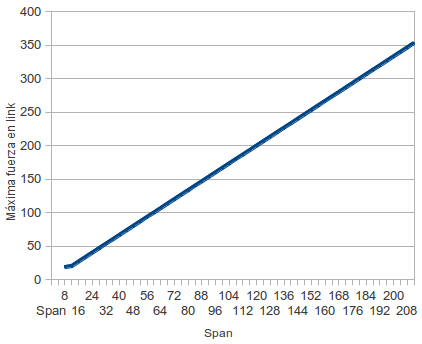
\includegraphics[scale=0.8]{archivos/graficos/Fuerza-x-span.png}
	\caption{\label{fig:fuerza_x_span}Fuerza máxima por Span de puente\\  \textit{Secciones}: $8$, \textit{altura}: $3$, \textit{peso de cargas}: $5$}
	\end{center}
\end{figure}

\begin{figure}[h!]
	\begin{center}
	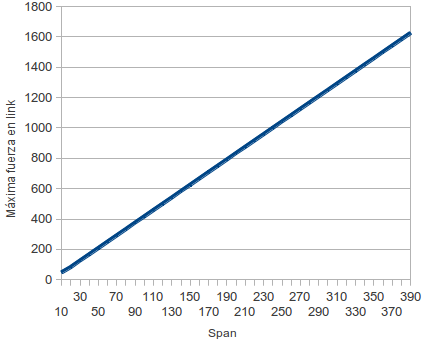
\includegraphics[scale=0.8]{archivos/graficos/Fuerza-x-span2.png}
	\caption{\label{fig:fuerza_x_span2}Fuerza máxima por Span de puente\\  		\textit{Secciones}: $8$, \textit{altura}: $3$, \textit{peso de cargas}: $5$}
	\end{center}
\end{figure}

En las figuras \ref{fig:fuerza_x_span} y \ref{fig:fuerza_x_span2}, podemos observar que la máxima fuerza en algún link del puente crece linealmente conforme aumenta el $span$. Es interesante notar que en los primeros dos casos, donde el ratio de \textit{ancho vs. altura} no supera $0,5$ la máxima fuerza es la compresión que reciben los links diagonales de los extremos, que soportan el peso completo del puente. De ahi en adelante la máxima fuerza es la compresión sufrida por los links centrales superiores.\\

Conforme las secciones del puente se hacen más anchas, esa carga aumenta linealmente, indicando que estas vigas soportan el mayor nivel de compresión y fuerza, y el análisis de costo de un puente deberia tomar este hecho en cuenta.\\

\subsubsection{Distribución de la cantidad de fuerzas}

Analicemos ahora la distribución de la cantidad de fuerzas en los casos cuando el \textit{span} es $200$ y $400$. En la figura \ref{fig:hist_fuerzas} el set de datos será: \textit{segmentos: 20}, \textit{altura: 3} y \textit{carga por sección: 5} para $i \in [1 \dots 19]$, y en \ref{fig:hist_fuerzas2}, observamos el comportamiento de un puento con la misma altura y peso, pero dos veces más largo.

\begin{figure}[h!]
\begin{center}
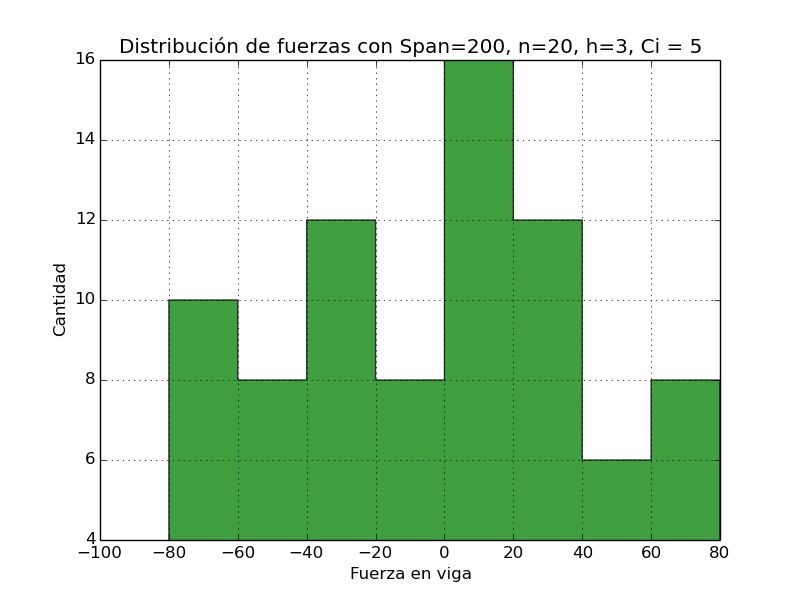
\includegraphics[scale=0.5]{archivos/graficos/hist_200.png}
\caption{\label{fig:hist_fuerzas}Histograma de distribución de fuerzas\\
\textit{Span}: $200$, $n$: $20$, $h$: $3$, $C_i$: $5$}
\end{center}
\end{figure}

\begin{figure}[h!]
\begin{center}
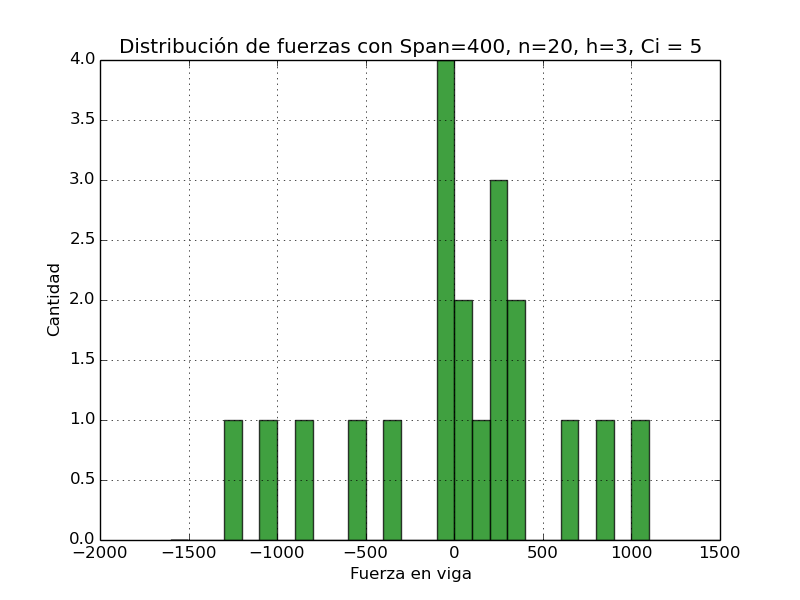
\includegraphics[scale=0.5]{archivos/graficos/hist_400.png}\\
\caption{\label{fig:hist_fuerzas2}Histograma de distribución de fuerzas\\
\textit{Span}: $400$, $n$: $20$, $h$: $3$, $C_i$: $5$}
\end{center}
\end{figure}

Comparando ambos gráficos se puede ver que la fuerza de las juntas se concentra
en la cercanía a $0$, y luego las fuerzas se distribuyen uniformemente hacia los extremos. Analizando los resultados emitidos por el programa, resulta que los links verticales y diagonales son los que suelen sufrir las menores fuerzas, y el grueso de las fuerzas internas afectan a los segmentos horizontales.

Es interesante notar que la distribución de fuerzas es similar en ambos casos; lo único que cambia es la magnitud de las fuerzas, que, como vimos en \ref{fig:fuerza_x_span} y \ref{fig:fuerza_x_span2}, incrementa linealmente.

\subsection{Experimento 2: Aumentar el span, pero fijando una carga central}

Ahora veamos qué sucede cuando aumentamos el $span$, dejando todo fijo pero
 colocando solamente un peso significativo en la junta central y fijando las restantes en $0$.\\

\begin{figure}[h!]
\begin{center}
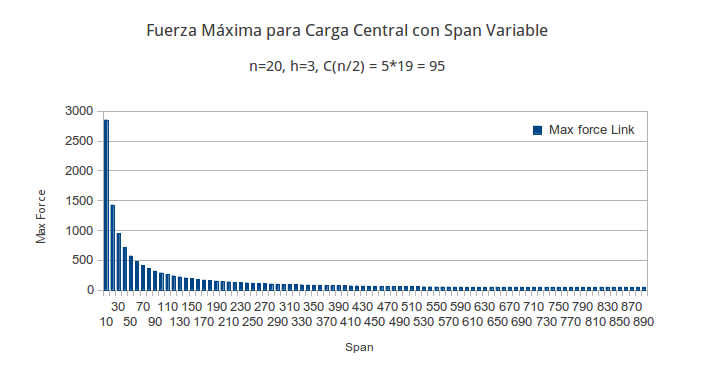
\includegraphics[scale=0.8]{archivos/graficos/Fuerza-x-span-peso-central.png}
\caption{\label{fig:fuerza_x_span_peso_central}Fuerza máxima por Span de puente con carga central\\
\textit{Secciones}: $20$, \textit{altura}: $3$, \textit{peso total}: $5 * 19 = 95$}
\end{center}
\end{figure}

Cuando ponemos el peso equivalente a la carga distribuida uniformemente en el
vértice central, notamos que el comportamiento es idéntico al experimento
anterior en forma, pero la fuerza máxima soportada por un link es considerablemente mayor, y el valor del span desde el cual la fuerza máxima es soportada por los links diagonales exteriores es mayor (cuando $span = 600$).\\

Esto se explicaría porque la distribución centralizada del peso fuerza a que los links centrales concentren las fuerzas de la carga sin la ayuda de los links más distantes del centro del puente, que juegan un mayor rol cuando el peso es más uniforme.

\newpage
\subsection{Experimento 3: Cambiar la cantidad de secciones}

Ahora analizamos cómo se comportan las fuerzas de los links cuando cambiamos la cantidad de secciones en los que está subdividido.\\

En las figuras \ref{fig:hist_n100_C100} y \ref{fig:hist_n10_C100}, generamos un puente de longitud $100$, con el primer caso teniendo $100$ secciones, y en el segundo caso, solo $10$.

\begin{figure}[h!]
\begin{center}
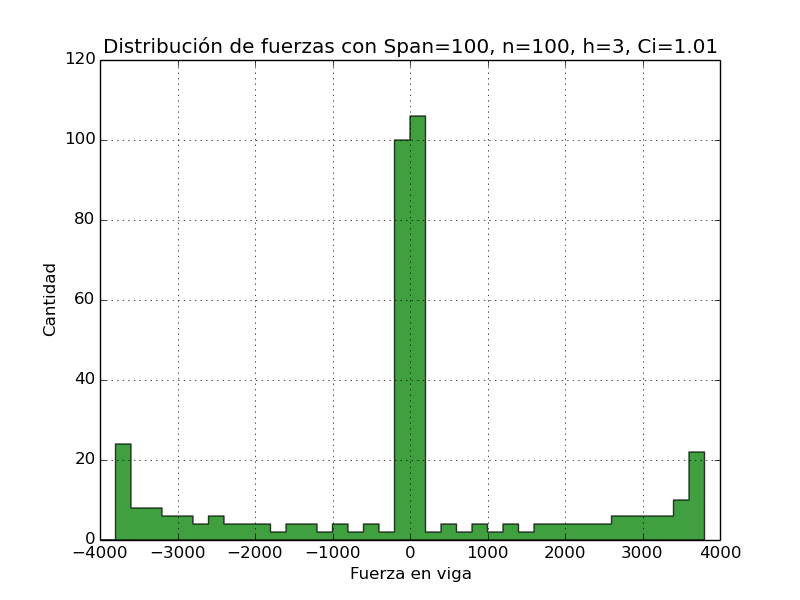
\includegraphics[scale=0.5]{archivos/graficos/hist_n100_C100.png}
\caption{\label{fig:hist_n100_C100}Histograma de distribución de fuerzas\\
\textit{span}=$100$, $n=100$, $h=3$, $C_i=1,01$}
\end{center}
\end{figure}

\begin{figure}[h!]
\begin{center}
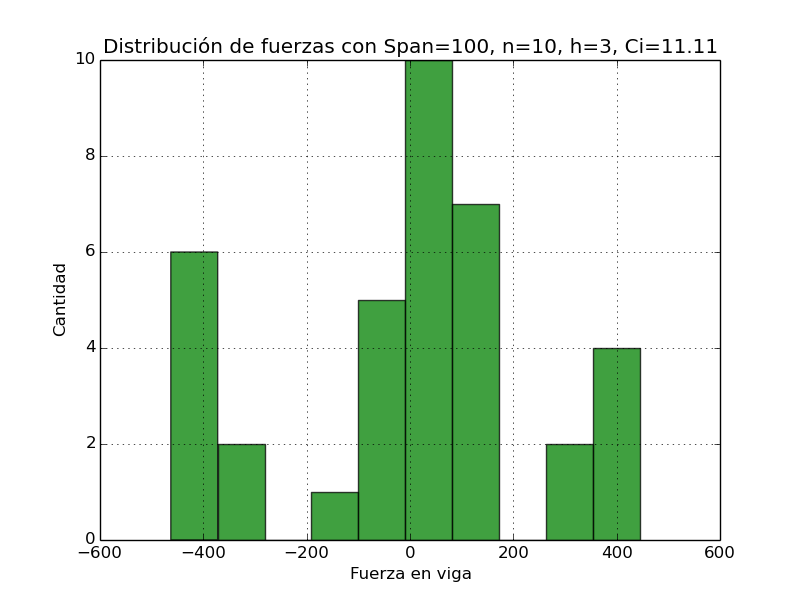
\includegraphics[scale=0.5]{archivos/graficos/hist_n10_C100.png}
\caption{\label{fig:hist_n10_C100}Histograma de distribución de fuerzas\\
\textit{span}=$100$, $n=10$, $h=3$, $C_i=11,11$}
\end{center}
\end{figure}

\begin{figure}[h!]
\begin{center}
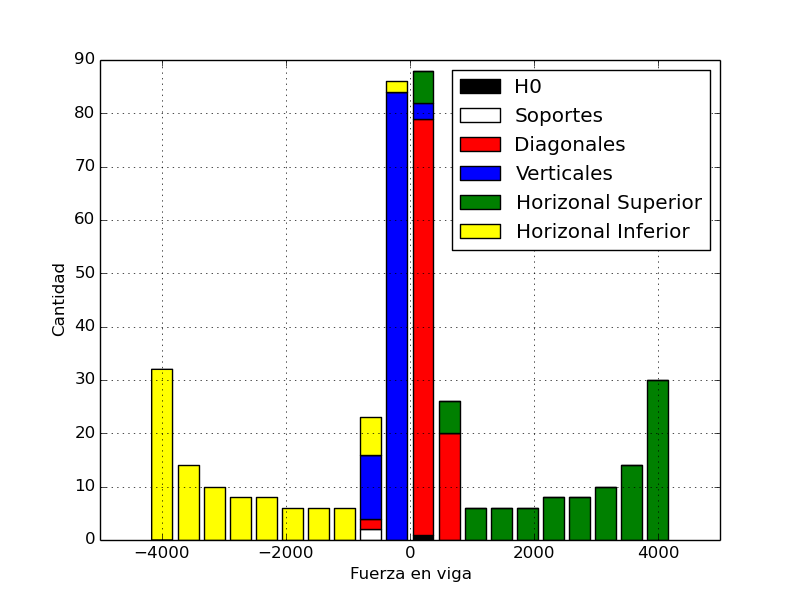
\includegraphics[scale=0.5]{archivos/graficos/hist_n100_C1000.png}
\caption{\label{fig:hist_n100_C1000}Histograma de distribución de fuerzas\\
\textit{span}=$100$, $n=100$, $h=3$, $C_i=10,10$}
\end{center}
\end{figure}

\begin{figure}[h!]
\begin{center}
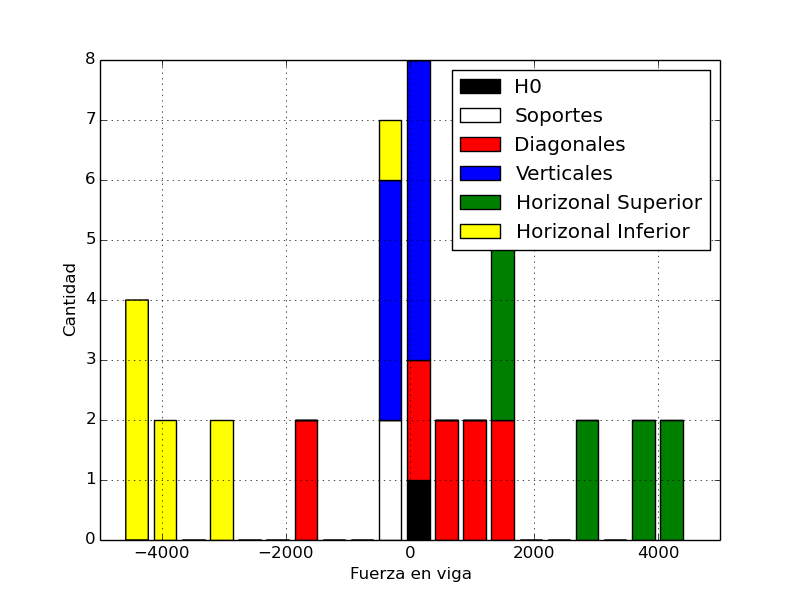
\includegraphics[scale=0.5]{archivos/graficos/hist_n10_C1000.png}
\caption{\label{fig:hist_n10_C1000}Histograma de distribución de fuerzas\\
\textit{span}=$100$, $n=10$, $h=3$, $C_i=111.11$}
\end{center}
\end{figure}

Observamos que la máxima fuerza en los puentes densos y esparsos de misma longitud son similares, con el puente con menos links teniendo, en proporción levemente más links en los extremos, y las diagonales soportando un poco más de carga, aunque igualmente más cerca del cero que de los valores extremos.\\

Nótese que en el caso donde \textit{span}$=100$ y $n=10$, cada sección tiene una longitud de $10$ y altura de $3$ (es decir, es más ancha que alta), y cuando \textit{span}$=100$ y $h=100$, las mismas son rectangulares pero más altas que anchas.\\

Desde un punto de vista de costo y eficiencia en términos de utilización de material, la opción de usar menos links y tener secciones más anchas resulta preferible por sobre la inversa.\\

\subsubsection{Estudio con cargas asimétricas}
Probamos también aumentar el \textit{span} con carga asimétrica con \textit{número de secciones} $=20$, poniendo pesos en los links inferiores de las secciones $4$ y $5$. Observamos que el comportamiento sigue siendo el mismo que en las figuras anteriores (es decir, una fuerza máxima grande que aumenta linealmente sobre el \textit{span}) relativo a la fuerza máxima, salvo que la misma ahora está situada en las secciones superiores directamente encima de los pesos.\\

Esto se explica debido a que los pesos flexionan el puente hacia abajo, y por ende los links superiores a los pesos sufren un efecto de compresión que permite que la estructura permanezca estable. Dado que en esta prueba el único cambio sobre las anteriores es que el peso está distribuido asimétricamente y en forma concentrada, es razonable que la estructura se siga comportando físicamente con el mismo patrón.\\

La figura \ref{fig:hist_asim} muestra la distribución de fuerzas en los links discriminada por tipo de link. Tal como analizamos en casos anteriores, las fuerzas diagonales y verticales son relativamente bajas en el espectro total, mientras que los extremos son dominados por las fuerzas horizontales, con las superiores sufriendo compresión, y las inferiores, tensión.

\begin{figure}[h!]
\begin{center}
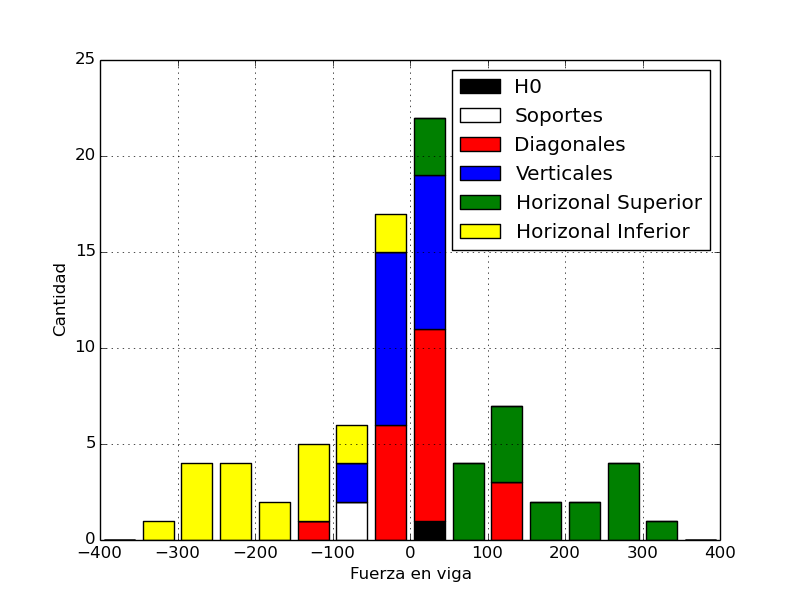
\includegraphics[scale=0.5]{archivos/graficos/hist_asim.png}
\caption{\label{fig:hist_asim}Detalle de distribución de fuerzas\\
\textit{span}=$60$, $n=10$, $h=3$, $C_i$ \textit{asimétrico}}
\end{center}
\end{figure}



    \newpage
    \section{Discusión y Conclusiones}
% Se incluira aqu un analisis de los resultados obtenidos en la seccion
% anterior (se analizara su validez, coherencia, etc.). Deben analizarse como
% materianimo los lostems pedidos en el enunciado. No es aceptable decir que
% \los resultados fueron los esperados", sin hacer clara referencia a la
% teoremasa a la cual se ajustan. Ademas, se deben mencionar los resul- tados
% interesantes y los casos \patologicos" encontrados.

\subsection{Distribución de los pesos en las juntas}

A lo largo de los distintos experimentos que hicimos, nos llamó la atención que la asignación de los pesos no variaba en demasía las fuerzas ejercidas sobre los ejes.\\

Esto es claro verlo en los Experimentos 1 y 2 en donde variábamos la distribución de los pesos y las fuerzas disminuían análogamente en cada gráfico.

\subsection{Cantidad de secciones con $span$ fijo}

Se puede ver que para mayor cantidad de secciones las fuerzas aplicadas sobre cada link van siendo cada vez menos uniformes, haciendo que para algunos links la fuerza sea casi nula y para otros sea excesivamente alta.\\

Algo que al verlo nos pareció natural, pero que aún así no deja de llamarnos la atención, fue que en esta serie de gráficos de distribución de las fuerzas, la repartición de los links que estaban tensionados contra los que estaban en compresión fue casi simétrica. La diferencia, creemos, debe ser por errores numéricos.

\subsection{Los links centrales son los que soportan mas fuerzas}

Tal vez nos faltó agregar una serie de gráficos para hacer mas explícito este punto, pero podemos asegurar que en la mayoría de los casos observados pudimos comprobar que esto se cumplía.
    \newpage
    \section{Heurística}

En esta sección, utilizando las conclusiones de los experimentos anteriores, proponemos una heurística para resolver el particionamiento de un \textit{span} a cubrir con un puente en subpuentes soportados por pilares con un costo predeterminado.\\

\subsection{Enunciado de heurística}

Considerando el comportamiento predecible de las fuerzas del puente según los estudios preliminares, consideramos que una heurística que particiona el problema en subproblemas y los resuelve con resultado satisfactoriamente ``buenos'' deberia retornar resultados cercanos al óptimo global del problema. Esto es en esencia la definición de una heurística de tipo \textit{Divide and Conquer}.\\

Veamos primero el pseudocódigo de lo que hicimos y luego explicaremos brevemente su motivación.\\

\begin{verbatim}
def heuristica(m, begin, end, n):

    costo, f_max = calc_costo_fuerza(m, begin, end)

    if n == 2:
        return costo, None
    else:
        cost1, pilares = heuristica(m, 0, mitad(n))
        cost2, pilares2 = heuristica(m, mitad(n), n)
        costo_heuristica = cost1 + cost2 + costo_pilar

    // Si se rompe o sale más barato dividir
    if f_max > f_limite or (cost1 + cost2 + costo_pilar < costo):
        poner_pilar(n/2)
        return costo_heuristica, (pilares + pilares2 + pilar[n/2])
    else:
        return (costo, None)
                        
def calc_costo_fuerza(m, inicio, fin)
    // Esta función devuelve el costo total del
    // subpuente y el valor de la máxima fuerza
    return costo, f_max
\end{verbatim}

En esencia, comparamos el costo de utilizar un puente para cubrir un \textit{span} vs. particionar el problema en 2, colocar un pilar en el medio, y poner dos puentes, y seleccionamos el caso óptimo. Esto se realiza recursivamente para cada subpuente, devolviendo  en cada etapa el mejor resultado de la heurística para la fracción calculada.

\subsection{Casos de prueba para Heurística}

A continuación enunciamos algunos casos de pruebas con los que verificamos el funcionamiento de la heurística, tanto para corroborar correctitud, casos regulares, y posibles casos patológicos.

\subsubsection{Caso de puente simple de 8 segmentos}
Una vez hechas la pruebas con puentes de 2 y 4 segmentos para verificar que la heurística funcionaba bien para casos extremadamente básicos, analizamos un puente simple de 8 segmentos con un peso centralizado importante y pesos uniformes bajos, y redujimos el costo de agregar un pilar hasta ver que la heurística considere pertinente agregar un pilar.\\

Observamos que, tal como es de esperar, le heurística prioriza agregar pilares con cercanía al peso más pesado. Si el costo de los pilares se reduce lo suficiente, se empiezan a agregar pilares soportando el resto de las secciones.

\subsubsection{Casos patológicos}

Una consecuencia del funcionamiento de la heurística es que, como fracciona el problema en subproblemas sin contemplar las interacciones entre las distintas subsecciones, no puede contemplar el abanico completo de posiciones en las que puede colocar un pilar. De ahi es posible que ocurran casos patológicos donde no se contemplan opciones que, siendo cercanas a las que pueden generar, produce resultados mucho mejores. Ilustramos esto con el siguiente ejemplo:\\

Tenemos un puente con los siguientes parámetros: \textit{span}:$40$, $h$:$4$, $n$:$20$, \textit{costo por pilar}: $5000$, \textit{max\_carga}: $2000$ y las cargas:\\

\begin{verbatim}
5
5
5
5
5
5
5
5
50
50
50
5
5
5
5
5
5
5
5
\end{verbatim}

El resultado emitido por la heurística, según el formato de la cátedra, es:\\

\begin{verbatim}
1
10
10399.3
10399.3
\end{verbatim}

Podemos observar que, razonáblemente, colocó un pilar entre una de las tres cargas de peso 50, pero ninguna de las configuraciones posibles de la heurística permitian generar un resultado mejor.\\

Observemos ahora el resultado que ocurre si desplazamos las cargas de $50$ un elemento hacia abajo:

\begin{verbatim}
3
6
8
10
2506.23
215.998
2159.98
7295.08
\end{verbatim}

El resultado muestra que se colocaron pilares en posiciones que son evidentemente mucho más óptimas, y esto se debe a que la heurística contempló los pesos concentrados de tal forma en que las dos subsecciones del problema que las abarca daban mejores resultados.\\

Lamentablemente, la diferencia es significativa: el primer resultado es $1,7$ veces mayor que el segundo, si bien es claro que con un poco de prueba y error se podría obtener un resultado mucho mejor dada la similitud de los casos.\\


    \newpage
    \section{Conclusiones}

En este trabajo practico realizamos el estudio de puentes tipo Pratt Truss. Nuestro análisis se enfocó en el estudio de las fuerzas que sufren los links en los puentes conforme se alteraban distintos parámetros.\\

\subsection{Conclusiones del análisis de puentes}

Habiendo hecho los estudios anteriores, podemos concluir que el comportamiento de las estructura es, en general, bastante predecible en cuanto a las fuerzas ejercidas en el puente.\\

Alterar la posición o distribución de fuerzas en el puente no exhibe cambios en el comportamiento estructural de las fuerzas; siguen apareciendo los mismos patrones de compresión y tensión que observamos en todos los casos de prueba.\\

Hay dos conclusiones importantes a la hora de considerar los costos asociados a un puente que debe cubrir un cierto \textit{span}:

\begin{itemize}
\item Al fraccionar un puente en más secciones no observamos que necesariamente se produzcan mejoras en el máximo valor absoluto de alguna fuerza del puente. Si bien esto amerita más estudio, se puede generalizar que, para la ecuación de costo provista por la cátedra, es preferible minimizar la cantidad de links dentro de un parámetro razonable.
\item La cantidad de fuerzas cerca del máximo valor absoluto es reducida. En la práctica esto se puede traducir a que se podría, en la realidad, experimentar con materiales de mayor integridad estructural para las juntas críticas horizontales, y otros de menor costo para las fuerzas diagonales y verticales (con la excepción de las diagonales extremas, que soportan el peso del puente).
\item Los comportamientos de fuerzas en relación a aumentos de fuerzas para cambios de dimensiones y cargas suelen exhibir una naturaleza lineal. Es decir, observamos que duplicar alguno de los parámetros del puente estudiados (por ejemplo, peso total, \textit{span} o $n$) incrementarán las fuerzas internas en un factor lineal. Esto quiere decir que es improbable, dados los casos de estudio, que existan otros casos patológicos donde el comportamiento del puente sea muy distinto.
\end{itemize}

Respecto al código que resuelve el problema, encontramos que las soluciones que generaban sufren de una cierta inestabilidad numérica en comparación al método de resolución de \textit{NumPy}, que internamente realiza una descomposición $P * L * U$ de la matriz e invoca métodos extremadamete refinados de librerias \textit{BLAS} con décadas de investigación. No obstante, nos llama la atención que la imprecisión es significativa (a lo sumo $1\%$) si bien la implementación es una copia directa de métodos propuestos por Burden.

\subsection{Conclusiones de la heurística}

La heurística presentada tiene un par de ventajas considerables: tiene una implementación simple con funcionamiento fácil de verificar y terminación clara, al particionar el problema de optimización hasta llegar a un caso base. Además, su tiempo de ejecución es extremadamente rápido.\\

No obstante, encontramos que la misma sufre de ciertas desventajas:\\

\begin{itemize}
\item La heurística solo puede elegir, para cada subproblema, entre el costo de un puente de longitud total o la solución para los dos subproblemas, particionados por la mitad de secciones del problema. Esto acota el espacio de solución posible y omite muchas soluciones potencialmente buenas.
\item El hecho de que las particiones de subproblemas están aisladas implica que no se pueden contemplar optimizaciones que deberia analizar ambas partes del subproblema en conjunto. Esto genera casos patológicos que serian fácilmente resolubles analizando subproblemas de otras formas, o usando heurísticas que analicen el puente en su totalidad.
\end{itemize}

\subsection{Trabajo futuro}
Proponemos el siguiente trabajo futuro basado en los resultados, conclusiones y experiencias obtenidas a lo largo del desarrollo de este trabajo:

\begin{itemize}
\item Optimizar la implementación. Si bien en términos de almacenamiento la matriz esparsa resulta una buena elección, las triangulación por eliminación gaussian tiene una variedad enorme de posibles implementaciones más rápidas y más precisas.
\item Analizar los efectos de la altura del puente. Si bien analizar $span$ para cargas fijas se puede considerar equivalente, un estudio más detallado del mismo nos podria haber dado resultados incluso más conclusivos sobre cómo evolucionan los costos y fuerzas del puente.
\item Comparar el puente Pratt Truss a otros puentes Truss. La literatura menciona una variedad enorme de puentes Truss, todos con distintas ventajas y desventajas, y algunos contemplados para ciertos perfiles de fuerzas y materiales disponibles.
\item Explorar la heurística más a fondo. A simple vista un eje para refinar la misma podría consistir en estudiar distintas formas de particionar los subproblemas y comparar los respectivos costos. Esto incrementaría el \textit{runtime} del problema, pero probablemente mejoraría muchísimo el resultado sin tener que recurrir a otros métodos más complejos.
\end{itemize}

    \newpage
    \section{Anexos}
\subsection{Pseudocodigo de metodos}
copiar pseudocodigo (comentarios) de %newton_start newton_iter secante_start
%secante_iter y loop principal

\subsection{Detalle de experimentos}

en este anexo detallamos los diferentes experimentos, como replicarlos y la
motivacion detras de cada uno de ellos.

por cada experimento indicar en que archivo esta, y que corridas se hicieron
con que datos y por que elegimos hacer ese exp.

    \appendix
% En el apendice A se incluira el enunciado del TP. En el apendice B se
% incluiran los codigos fuente de las funciones relevantes desde el punto de
% vista numerico. Resultados que valga la pena mencionar en el trabajo pero que
% sean demasiado especicos para aparecer en el cuerpo principal del trabajo
% podran mencionarse en sucesivos apendices rotulados con las letras mayusculas
% del alfabeto romano. Por ejemplo: la demostracion de una propiedad que
% aplican para optimizar el algoritmo que programaron para resolver un
% problema.
%    \input{archivos/enunciado.tex}
    \section{Referencias}
% Es importante incluir referencias a libros, articleculos y paginas de
% Internet consultados durante el desarrollo del trabajo, haciendo referencia a
% estos materiales a lo largo del informe. Se deben citar tambien las
% comunicaciones personales con otros grupos

Wikipedia
Burden

    \section{Anexos}
\subsection{Pseudocodigo de metodos}
copiar pseudocodigo (comentarios) de %newton_start newton_iter secante_start
%secante_iter y loop principal

\subsection{Detalle de experimentos}

en este anexo detallamos los diferentes experimentos, como replicarlos y la
motivacion detras de cada uno de ellos.

por cada experimento indicar en que archivo esta, y que corridas se hicieron
con que datos y por que elegimos hacer ese exp.

\end{document}
